%%%%%%%%%%%%%%%%%%%%%%%%%%%%%%%%%%%%%%%%%%%%%%%%%%%%%%%%%%%%%%%%%%%%%%
% amspaper.tex --  LaTeX2e-based template for submissions to American 
% Meteorological Society Journals, including
%
% JAS 	-- Journal of the Atmospheric Sciences
% JAMC 	-- Journal of Applied Meteorology and Climatology
% JPO 	-- Journal of Physical Oceanography
% MWR 	-- Monthly Weather Review
% JTECH -- Journal of Atmospheric and Oceanic Technology
% WAF 	-- Weather and Forecasting
% JCLI 	-- Journal of Climate
% JHM 	-- Journal of Hydrometeorology
% JAM 	-- Journal of Applied Meteorology
%
% Template developed by B. Papa and S. Cooley, AMS. 
% Email questions to latex@ametsoc.org.
%
% August 12, 2008 (SRC)
%	- Clarified/added header notes, comments throughout
%	- Improved title page
%	- Edited text of document for clarity
%	- Altered list styles to adhere to AMS style, added comments
%	- Removed incorrect commands (i.e., \catcode) (corrects umlaut bug)
%	- Moved non-template commands to ametsoc.sty
%
% August, 2008 - B. Papa
% - Updated to handle two column journal page output
% - Updated text with new/modified instructions
%
%%%%%%%%%%%%%%%%%%%%%%%%%%%%%%%%%%%%%%%%%%%%%%%%%%%%%%%%%%%%%%%%     
%%%%%%%%%%%%%%%%%%%%%%%%%%%%%%%%%%%%%%%%%%%%%%%%%%%%%%%%%%%%%%%%
%																															 %
%				USE THIS TEMPLATE, AMETSOC.STY, AND AMETSOC.BST				 %
%			        OR YOUR TEX FILES WILL NOT BE USED				  		 %
%																															 % 
%%%%%%%%%%%%%%%%%%%%%%%%%%%%%%%%%%%%%%%%%%%%%%%%%%%%%%%%%%%%%%%%
%%%%%%%%%%%%%%%%%%%%%%%%%%%%%%%%%%%%%%%%%%%%%%%%%%%%%%%%%%%%%%%%

%%%%%%%%%%%%%%%%%%%%%%%%%%%%%%%%%%%%%%%%%%%%%%%%%%%%%%%%%%%%%%%%%%%%%
% PREAMBLE
%%%%%%%%%%%%%%%%%%%%%%%%%%%%%%%%%%%%%%%%%%%%%%%%%%%%%%%%%%%%%%%%%%%%%
%
% The following two commands will generate a PDF that follows all the requirements for submission
% and peer review.  Uncomment these commands to generate this output (and comment out the two lines below.)
%
% DOUBLE SPACE VERSION FOR SUBMISSION TO THE AMS
\documentclass[12pt]{article}
\usepackage{ametsoc}
%
% The following two commands will generate a single space, double column paper that closely
% matches an AMS journal page.  Uncomment these commands to generate this output (and comment
% out the two lines above. FOR AUTHOR USE ONLY. PAPERS SUBMITTED IN THIS FORMAT WILL BE RETURNED
% TO THE AUTHOR for submission with the correct formatting.
%
% TWO COLUMN JOURNAL PAGE LAYOUT FOR AUTHOR USE ONLY
%\documentclass[10pt]{article}
%\usepackage{ametsoc2col}
\usepackage{subfigure}
\usepackage{comment}
%
%%%%%%%%%%%%%%%%%%%%%%%%%%%%%%%%%%%%%%%%%%%%%%%%%%%%%%%%%%%%%%%%%%%%%
% ABSTRACT
%
% Enter your Abstract here
%%%%%%%%%%%%%%%%%%%%%%%%%%%%%%%%%%%%%%%%%%%%%%%%%%%%%%%%%%%%%%%%%%%%%
\newcommand{\myabstract}{The Limited Area Model (LAM) forecasting problem is not only an initial condition problem but also a lateral boundary condition (LBC) problem. The lateral boundary conditions are generally provided by a host model, for example the forecast of a global numerical weather prediction (NWP) model or a forecast with a larger model domain. The purpose of data assimilation in numerical weather prediction is to combine the real-time and/or past observations with the forecast from a NWP model to produce the analysis, which is considered "the best" estimate of the current state of the system,to be used for the subsequent forecasts. In the four-dimensional variational data assimilation (4D-Var) system of Weather Research and Forecasting (WRF) model, in addition to the control of the initial conditions, the lateral boundary conditions are is also controlled during the minimization to completely take into account the impact of observations close to the lateral boundaries. Considering the control of the lateral boundary conditions in 4D-Var is particularly important for assimilating phenomena close to inflow boundary that are well observed during the later part of the assimilation window. If we do not control the lateral boundary conditions, observed information related to such phenomena may be lost.}
%
\begin{document}
%
%%%%%%%%%%%%%%%%%%%%%%%%%%%%%%%%%%%%%%%%%%%%%%%%%%%%%%%%%%%%%%%%%%%%%
% TITLE
%
% Enter your TITLE here
%%%%%%%%%%%%%%%%%%%%%%%%%%%%%%%%%%%%%%%%%%%%%%%%%%%%%%%%%%%%%%%%%%%%%
\title{\textbf{\large{Control of lateral boundary conditions in WRF 4D-Var}}}
%
% Author names, with corresponding author information. 
% [Update and move the \thanks{...} block as appropriate.]
%
\author{\textsc{Xin Zhang}
				\thanks{\textit{Corresponding author address:} 
				Dr. Xin Zhang, NCAR/MMM, P.O. Box 3000, 
				 Boulder, CO 80307. 
				\newline{E-mail: xinzhang@ucar.edu}}\\
\textit{\footnotesize{National Center for Atmospheric Research, Boulder, Colorado 80307}}
\and 
\centerline{\textsc{Nils Gustafsson}}\\% Add additional authors, different institution
\centerline{\textit{\footnotesize{Swedish Meteorological and Hydrological Institute, SE-60176 Norrk�oping, Sweden}}}
\and
\centerline{\textsc{Xiang-Yu Huang}}\\% Add additional authors, different institution
\centerline{\textit{\footnotesize{National Center for Atmospheric Research, Boulder, Colorado 80307}}}
}
%
% The following block of code will handle the formatting of the title page depending on whether
% we are formatting a double column (dc) author draft or a single column paper for submission.
% AUTHORS SHOULD SKIP OVER THIS... There is nothing to do in this section of code.
\ifthenelse{\boolean{dc}}
{
\twocolumn[
\begin{@twocolumnfalse}
\amstitle

% Start Abstract (Enter your Abstract above.  Do not enter any text here)
\begin{center}
\begin{minipage}{13.0cm}
\begin{abstract}
	\myabstract
	\newline
	\begin{center}
		\rule{38mm}{0.2mm}
	\end{center}
\end{abstract}
\end{minipage}
\end{center}
\end{@twocolumnfalse}
]
}
{
\amstitle
\begin{abstract}
\myabstract
\end{abstract}
\newpage
}
%%%%%%%%%%%%%%%%%%%%%%%%%%%%%%%%%%%%%%%%%%%%%%%%%%%%%%%%%%%%%%%%%%%%%
% MAIN BODY OF PAPER
%%%%%%%%%%%%%%%%%%%%%%%%%%%%%%%%%%%%%%%%%%%%%%%%%%%%%%%%%%%%%%%%%%%%%
%
\section{Introduction}
The four-dimensional variational data assimilation (4D-Var) technique (Le Dimet and Talagrand 1986; Lewis and Derber 1985) has been pursued actively by the research community and operational centers over the past two decades. The first successful operational 4D-Var system was implemented at the European Centre for Medium-Range Weather Forecasts (ECMWF) using an incremental formulation (Courtier et al. 1994; Rabier et al. 1997). The results demonstrate a significant positive impact on operational forecasts compared to its 3D-Var system (Rabier et al. 2000). Following ECMWF, several operational centers implemented 4D-Var in their operational applications, including Meteo-France (Gauthier and Thepaut 2001), the Met Office (Lorenc and Rawlins 2005; Rawlins et al. 2007), the Japan Meteorological Agency (Honda et al. 2005), and Environment Canada (Gauthier et al. 2007). Other operational centers are also preparing 4D-Var as their data assimilation package, including the High-Resolution Limited-Area Model community (HIRLAM; Huang et al. 2002) and the Naval Research Laboratory Atmospheric Variational Data Assimilation System (NAVDAS-AR; Xu et al. 2005).

The success of the global 4D-Var system in improving global forecasts provided enough encouragement to go ahead with a regional 4D-Var for mesocale and thunderstorm scales. Several regional 4D-Var research systems have been developed, including 1) one based on the fifth-generation Pennsylvania State University National Center for Atmospheric Research (PSU� NCAR) Mesoscale Model (MM5; Zou et al. 1995, 1997; Ruggiero et al. 2006), 2) one based on the National Centers for Environmental Prediction (NCEP) Eta Model (Zupanski 1993), 3) the 4D-Var-based Regional Atmospheric Modeling System (RAMS) data assimilation system (RAMDAS; Zupanski et al. 2005), and 4) the variational Doppler Radar assimilation system (VDRAS) for convective-scale assimilation of radar data (Sun and Crook 1997); 5) the Japan Meteorological Agency (JMA) 4D-Var system (Meso-4DVAR; Koizumi et al. 2005) and NHM-4DVAR (\cite{Kawa2007}), 6) a 4D-Var system for the High Resolution Limited Area Model (HIRLAM) forecasting system (\cite{Gustafd2011}), 7) a 4D-Var system for the Weather Research and Forecasting model (WRF) (\cite{Huang2009}).

The Limited Area Model (LAM) or regional forecasting problem is a lateral boundary condition problem in addition to the initial condition problem. For 
numerical weather prediction, the lateral boundary conditions are generally provided by a host model, for example a global numerical weather prediction 
model. There is much evidence that, for some widely used combinations of domain size and forecast period, forecasts are more sensitive to the LBC specification than to the initial condition (IC) specification within the model domain (Vukicevic and Errico, 1990). This is to be expected because as time advances, features are advected from inflow boundaries into the interior and interior features exit at the outflow boundaries. For regional 4D-Var , the cost function is a function of the initial condition and the lateral boundary condition. 
\begin{comment}
As a starting point, one may that the available boundary conditions from the host model have to be accepted (without change) for usage in the LAM. However, one may use the observations close to the lateral boundaries and let these influence the initial conditions. In case the initial conditions are used as the lateral boundary conditions at the initial time, the subsequent forecast will also be influenced by these observations. Depending on the frequency of the 
updating of the lateral boundary conditions, the host model will gradually take over the definition of the lateral boundary conditions.
\end{comment}

For the control of the lateral boundary conditions in a LAM 4D-Var data assimilation, the tangent linear and adjoint versions of the schemes for the coupling to the larger scale model providing the lateral boundary conditions are needed. \cite{Errico1993} applied the adjoint of the model and its LBC formulation in a limited area model to investigate the sensitivity of limited area model forecast errors to initial as well as lateral boundary conditions. Their research suggested that sensitivity with respect to LBC increases sharply at the time a feature of significant IC sensitivity impacts with the LBC region, and the IC sensitivity may decrease sharply although not disappear entirely.  They also pointed out that the time at which sensitivity with respect to a LBC field has greater magnitude than for a corresponding IC field will be later for a winter case than for a summer case.  A similar study was carried out by \cite{Gusta1998} for a significant storm development over the North Atlantic, indicating that errors in initial as well as in lateral boundary conditions may explain some forecast failures and the sensitivity experiments with respect to the lateral boundary conditions indicate that poor quality lateral boundary conditions may be improved by utilizing subsequent downstream observations within the model integration area. This result may be directly applied in 4D-Var and during the assimilation period the boundary values can be modified together with modifications in the initial state.

With application of 4D-Var for the LAM forecasting, one may control the lateral boundary conditions during the period of the data assimilation window. This may be particularly important for assimilation of phenomena that are observed well inside the LAM domain during the later part of the data assimilation window, while being propagated through the lateral boundaries during the early part of the data assimilation window. If we do not control the lateral boundary conditions, observed information related to these phenomena may be lost. For the control of the lateral boundary conditions in 4D-Var, in the Japan Meteorological Agency (JMA) mesoscale LAM 4D-Var, \cite{Kawa2007} introduced a full model state control variable for the lateral boundary conditions at the end of the assimilation window and a 4D-Var cost function constraint for this new lateral boundary control variable, with a similar form as for the background error constraint. \cite{Gusta2011} follows the JMA approach to control LBC in the HIRLAM 4D-Var and gets a positive impact on a winter storm case over the Scandinavia peninsula in Europe. In WRF 4D-Var, we also follow the JMA approach and we introduce a full model state control variable at the end of assimilation window for the lateral boundary control. The perturbations of model control variables at the start and the end of the assimilation window will be used to estimate the perturbations of the model variable lateral boundary tendencies. 

Recently, we re-developed the WRF tangent-linear model and adjoint model based on the latest repository WRF. Compared to the previous version of the WRF tangent-linear and adjoint models in Xiao et al 2009, \cite{Huang2009}, the LBC scheme has been carefully investigated and coded with the corresponding tangent-linear and adjoint LBC schemes. 

The purpose of this paper is to describe the implementation and impact of the LBC control in the WRF 4D-Var system. The formulation of the WRF 4D-Var and the newly developed WRF tangent linear and adjoint models are presented in section 2, followed by an example of implicit dynamic structure functions using single observation experiments in section 3 to demonstrate the validation of the LBC control in WRF 4D-Var. A comparison of forecasting performance for real observation data assimilation of a winter storm are described in section 4 in order to demonstrate the impact of the LBC control. The computational efficiency of the newly developed WRF 4D-Var is discussed in section 5 and some concluding remarks are given in section 6.

\section{The 4D-Var LBC Control Algorithm}

\subsection{Minimization algorithm}
The WRF 4D-Var algorithm takes the incremental 4D-Var formulation that is commonly used in operational systems (Courtier et al. 1994; Veerse and Thepaut 1998; Lorenc 2003). The incremental approach is designed to find the analysis increment that minimizes a cost function defined as a function of the analysis increment instead of the analysis itself. In the incremental 4D-Var, the tangent linear and adjoint models usually derived from a simplified forward model are used in the inner-loop minimization, while the evolution of the background is predicted with the full forward model. The current WRF 4D-Var system makes use of the following components of the previously developed WRF-Var system (Barker et al. 2005): 1) observation operators, 2) quality control, 3) the background error covariance model. The new developments specified for the current WRF 4D-Var system are : 1) a minimization inner-loop using newly developed simplified WRF tangent linear and adjoint models which will be briefly described later, and 2) an iterative outer loop using the nonlinear WRF model to update the basic trajectory state to account for the effect of nonlinearities in the assimilation algorithm.

The basic WRF 4D-Var system formulation can be found in \cite{Huang2009}. To take into account the constraint of the LBC in minimization, the WRF 4D-Var cost function $J$ turns out to be:
\begin{equation}
J(\mathbf{x}_\mathrm{0},\mathbf{x}_\mathrm{lbc})=J_\mathrm{b}+J_\mathrm{o}+J_\mathrm{c}+J_\mathrm{lbc}
\end{equation}
Compared to the equation (1) in \cite{Huang2009}, in addition to the initial conditions as control variables and basic quadratic measures of distance to the background, observation and balanced solution, the model lateral boundary conditions, $\mathbf{x}_\mathrm{lbc}$ is the new control variable and there is an additional term $J_\mathrm{lbc}$ which measures distance between the analyzed LBC and first guess LBC. It is very important to include the LBC as a control variable since the sensitivity of a forecast aspect with respect to a LBC field has greater magnitude than for a corresponding IC field in winter (\cite{Errico1993}). 

For the control of lateral boundary conditions in WRF 4D-Var, we follow \cite{Kawa2007} 
\begin{equation}
J_\mathrm{lbc}=\frac{1}{2}(\mathbf{x}_\mathrm{lbc}-\mathbf{x}^{\mathrm{b}}_\mathrm{lbc})^T\mathbf{B}^{'-1}(\mathbf{x}_\mathrm{lbc}-\mathbf{x}^{\mathrm{b}}_\mathrm{lbc})
\end{equation}
where $\mathbf{x}_\mathrm{lbc}$ is the lateral boundary condition at the end of the assimilation window, $\mathbf{x}^{\mathrm{b}}_\mathrm{lbc}$ is the first guess of the $\mathbf{x}_\mathrm{lbc}$. $\mathbf{B}^{'-1}$ is the background error covariance matrix for $\mathbf{x}_\mathrm{lbc}$. 


\subsection{Lateral boundary control}
For real-data cases, the specified boundary condition is primarily used in WRF and it is also referred to as relaxation or nudging, boundary condition. The specified lateral boundary condition for the coarse grid requires an external file, generated during the same pre-processing for the initial condition file. Let $\mathbf{x}$ be any prognostic model state variable having a lateral boundary entry, following \cite{Davis1977}
\begin{equation}
\frac{\partial{\mathbf{x}}}{\partial{t}}=F_1(\mathbf{x}_\mathrm{lbc}-\mathbf{x})-F_2\Delta^2(\mathbf{x}_\mathrm{lbc}-\mathbf{x})
\end{equation}
where $\Delta^2$ is a 5-point smoothing operator,$ F_1$ and $F_2$ are (nudging) 
weighting coefficients depending on the distance to the lateral boundary, and $\mathbf{x}_\mathrm{lbc}$ is the corresponding boundary value 
provided by the host model. $\mathbf{x}_\mathrm{lbc}$ is specified in the following form:
\begin{equation}
\mathbf{x}_\mathrm{lbc}(t)=\mathbf{x}_\mathrm{lbc}(t_0)+(t-t_0)\frac{\Delta{\mathbf{x}_\mathrm{lbc}}}{\Delta{t}}
\end{equation}
where $\mathbf{x}_\mathrm{lbc}(t_0)$ is the starting point value along the domain boundary relaxation region and $\frac{\Delta\mathbf{x}_\mathrm{lbc}}{\Delta{t}}$ is the corresponding temporal tendency.

For the WRF model, if the LBC update interval is $t_i$ (such as 3h or 6h), then the temporal tendency of $\mathbf{x}$ from $t_{k-1}$ to $t_k$ is calculated as
\begin{equation}
\frac{\Delta{\mathbf{x}_\mathrm{lbc}}}{\Delta{t}}=\frac{\mathbf{x}_\mathrm{lbc}(t_k)-\mathbf{x}_\mathrm{lbc}(t_{k-1})}{t_k-t_{k-1}}
\end{equation}
From equation (3) and (4), we will see that $\mathbf{x}_\mathrm{lbc}(t)$ will depend on $\mathbf{x}_\mathrm{lbc}(t_k)$ and $\mathbf{x}_\mathrm{lbc}(t_{k-1})$, with $t_{k-1}\le{t}\le{t_k}$.

Therefore, considering a data assimilation window from time $t_{k-1}$ until time $t_k$ and it is presently required for WRF 4D-Var that the assimilation window has exactly the same duration as the LBC update interval, we already have $\delta{\mathbf{x}}(t_{k-1})$ ($\delta\mathbf{x}_\mathrm{lbc}(t_{k-1})$) at the start of the window as a assimilation control variable. If we add $\delta{\mathbf{x}}(t_k)$ ($\delta\mathbf{x}_\mathrm{lbc}(t_{k})$) as  another set of assimilation control variables, the quantities needed for the LBC in equation (3) of the tangent linear WRF model are given by
\begin{equation}
\delta{\mathbf{x}}_\mathrm{lbc}(t_{k-1})=\delta{\mathbf{x}}(t_{k-1})
\end{equation}
\begin{equation}
\delta{\mathbf{x}}_\mathrm{lbc}(t_{k})=\delta{\mathbf{x}}(t_{k})
\end{equation}
\begin{equation}
\delta\frac {{\Delta{\mathbf{x}}_\mathrm{lbc}}} {\Delta{t}}=\frac{\delta{\mathbf{x}}_\mathrm{lbc}(t_k)-\delta{\mathbf{x}}_\mathrm{lbc}(t_{k-1})} {t_k-t_{k-1}}
\end{equation}

\begin{comment}
Introduce the lateral boundary condition perturbations as a control variable $\delta{\mathbf{x}_\mathrm{lbc}}(t_k)$  at the end of the data assimilation window (time $t_k$).  For the lateral boundary increment $\delta{\mathbf{x}_\mathrm{lbc}}(t_0)$ at the start of the assimilation window (time $t_0$) we will use the initial condition increment $\delta{\mathbf{x}}(t_0)$. For intermediate time-steps during the integration of the tangent linear model, we will obtain the lateral boundary conditions by the same linear time interpolation scheme that is used in the non-linear model. Once the lateral boundary conditions are defined, the same lateral boundary relaxation scheme, see \cite{Davis1983}, that is used in the non-linear model can also be used in the tangent-linear model, and the adjoint of the lateral 
boundary relaxation is well defined, see \cite{Gusta1998}. Note however, that while the lateral boundary conditions are input data to the tangent linear model, the lateral boundary conditions are output data from the adjoint model. 
\end{comment}

The lateral boundary conditions input to the adjoint model at the end of the assimilation window are $\mathbf{x}_\mathrm{lbc}^\mathrm{ad}(t_k)$ and $(\frac {\Delta{\mathbf{x}}_\mathrm{lbc}} {\Delta{t}})^\mathrm{ad}$
, which will be initialized with zeroes. After the backwards integration of the adjoint model to 
time $t_{k-1}$ the adjoint control variables (or the error gradients) can be obtained 
from: 
\begin{equation}
\mathbf{x}_\mathrm{ic}^\mathrm{ad}(t_{k-1})=\mathbf{x}_\mathrm{ic}^\mathrm{ad}(t_{k-1})+\mathbf{x}_\mathrm{lbc}^\mathrm{ad}(t_{k-1})
\end{equation}
\begin{equation}
\mathbf{x}_\mathrm{ic}^\mathrm{ad}(t_{k-1})=\mathbf{x}_\mathrm{ic}^\mathrm{ad}(t_{k-1})-\frac{1}{t_k-t_{k-1}}(\frac{\Delta{\mathbf{x}_\mathrm{lbc}}}{\Delta{t}})^\mathrm{ad}
\end{equation}
\begin{equation}
\mathbf{x}_\mathrm{lbc}^\mathrm{ad}(t_k)=\frac{1}{t_k-t_{k-1}}(\frac{\Delta{\mathbf{x}_{lbc}}}{\Delta{t}})^\mathrm{ad}
\end{equation}
where $\mathbf{x}_\mathrm{ic}^\mathrm{ad}(t_{k-1})$ denotes the corresponding adjoint model variable of the IC within the relaxation region as provided at the initial time $t_{k-1}$.

Note that $\mathbf{x}_\mathrm{lbc}^\mathrm{ad}(t_{k-1})$ and $(\frac{\Delta{\mathbf{x}_\mathrm{lbc}}}{\Delta{t}})^\mathrm{ad}$ are defined in the boundary relaxtion 
zone only. Consider, however, that they are full domain fields that are 
initialized with zeroes at the end of the data assimilation window and that the boundary relaxation will only fill in values into this full domain 
field inside the boundary relaxation zone.

Also note that the calculation of $J_\mathrm{lbc}$ and $\frac{\partial{J_\mathrm{lbc}}} {\partial{\mathbf{v}_\mathrm{lbc}}}$, where $\mathbf{v}_\mathrm{lbc}$ is the lateral boundary condition control variable in control vector space, will follow exactly the same calculations as for the background error constraint. 

So for practical implementation, the cost function term $J_\mathrm{lbc}$ that quadratically measure the distance to the background LBCs at the end of assimilation window $t_k$ can be written
\begin{equation}
J_\mathrm{lbc}=J(\mathbf{x}(t_k))=\frac{1}{2}\delta{\mathbf{x}}(t_k)^T\bm{\mathbf{B}}_\mathrm{lbc}^{-1}\delta{\mathbf{x}}(t_k)
\end{equation}
where $\bm{\mathbf{B}}_\mathrm{lbc}$ represents the error covariance of the first guess LBCs at the end of the assimilation window. For WRF model, the coarse grid specified lateral boundary is comprised of both a specified and a relaxation zone (see WRF tech note in Fig. 6.1). The specified zone is determined entirely by temporal interpolation from an external forecast or analysis. The width of the specified zone is run-time configurable, but is typically set to 1. The second region of the lateral boundary for the coarse grid is the relaxation zone. The relaxation zone is where the model is nudged or relaxed towards the large-scale forecast. The size of the relaxation zone is also a run-time option and typically set to 4. Apparently, it is very difficulty to calculate and define the physical and statistical relationships in background error covariance just along several rows and columns of the lateral boundary relaxation region. It is practical that we take the whole model states at the end of assimilation window as the control variables and just use the model variables along lateral boundary relaxation region to calculate the lateral boundary conditions. Therefore, the $\bm{\mathbf{B}}_\mathrm{lbc}$ should take the same definition as $\bm{\mathbf{B}}$. As a reasonable assumption, we will apply $\bm{\mathbf{B}}_\mathrm{lbc}=\bm{\mathbf{B}}$ in our experiments. 

One may question whether the assumption of $\bm{\mathbf{B}}_\mathrm{lbc}=\bm{\mathbf{B}}$ is suitable because it is possible that high correlations may exist between the model state control variables at the start and end of the assimilation window. \cite{Gusta2011} takes statistics for vorticity as an example to check the differences between background forecast error statistics and forecast tendency error statistics estimated by NMC method. His estimation shows that the standard deviations for the forecast tendency differences are significantly larger than the standard deviations for full forecast differences in the middle troposphere and that the vorticity forecast differences are only weakly correlated over 5h in time. Therefore, for the 4D-Var with LBC control we may assume that the weak correlation in time of vorticity increments would make the minimization reasonably well conditioned.

\begin{comment}
One potential problem is that the introduction of the lateral boundary 
condition constraint in the form described above, would worsen the conditioning of the 4D-Var minimization problem, since the lateral boundary condition errors at the end of the assimilation window would be strongly 
correlated with the initial condition errors at the start of the assimilation 
window, at least for the large scale and slowly varying phenomena that are 
important for the lateral boundary conditions. One simple pre-conditioning 
would be to subtract the lateral boundary conditions at the start of the 
assimilation window from the lateral boundary conditions at the end of 
the assimilation window, thus to treat the tendency of the lateral boundary 
conditions 
\begin{displaymath}
(\frac{\partial{\delta{\mathbf{x}_\mathrm{lbc}}}}{\partial{t}})=\frac{\delta{\mathbf{x}_\mathrm{lbc}}(t_k)-\delta{\mathbf{x}_\mathrm{lbc}}(t_0)} {t_{k}-t_0}
\end{displaymath}
as the control variable. This approach would also require the covariance of forecast tendency errors, that possibly 
could be estimated by the NMC method from differences between forecast 
tendencies valid at the same time. 
\end{comment}

\subsection{Brief description of WRF tangent-linear and adjoint model}

NCAR started to develop its first version of the tangent-linear and adjoint models for the WRF ARW core around 2005 and research based on this version has been conducted and published such as in Xiao et al (2008), \cite{Huang2009} and Zhang Meng (2010). In the past few years, the WRF model and the WRF data assimilation (WRFDA) system have experienced extensive changes. However, the first version of WRF tangent-linear and adjoint model failed to catch up with the developments of the WRF and WRFDA systems and the out-dated tangent-linear and adjoint models lead to many problems when they were coupled with the latest WRF and WRFDA systems to become a 4D-Var system.

From the WRF model version 3.2 release, we started to re-develop the tangent-linear and adjoint models of WRF ARW core based on the latest WRF repository. Compared to its first version, the new version has following improvements: 1) Consistent with the latest WRF development, the current tangent-linear and adjoint codes are always kept up with the WRF changes; 2) Improved physics packages, in addition to vertical diffusion and surface drag, we also include a simplified microphysics scheme and a cumulus scheme;  3) More accurate and complete tangent-linear and adjoint checks are included to make sure that the existing codes and new developed codes are error free; 4) For the purpose of the lateral boundary control in regional 4D-Var and adjoint sensitivity analysis, the lateral boundary scheme was investigated carefully and its associated tangent-linear and adjoint codes were developed and checked, for details see Zhang et al. 2011.

\section{Single observation experiments with LBC control}
\label{sec:single}
Analysis increments due to a single observation produced by a data assimilation system implicitly provide the effective background error covariance matrix $\mathbf{B}$ and describe how the tangent linear and adjoint model propagate the observational information, see \cite{Huang2009}. After any new capability for the WRF 4D-Var system was developed, a single observation experiment is an effective and clean way to show the impact of the new capability on the analysis.

Given a single temperature observation at the end of the time window of 4D-Var, we knew that the 4D-Var increments have a temporal dimension, the increments at 6 h give a graphic representation of the background error covariance matrix at 6 h, $\mathbf{MBM}^T$, where $\mathbf{M}$ and $\mathbf{M}^T$ are the WRF tangent linear model and adjoint model, respectively. For the current regional WRF 4D-Var, both the initial condition and the lateral boundary conditions determine the future trajectory of the model. Therefore, the observations close to or within the lateral boundary relaxation region should not only impact the initial condition but also the lateral boundary condition.

%The first experiment has a single observation at 6 h, which is far from the lateral boundary and the tendency from LBC should have trivial or no impact on the observation location at 6 h, which means assimilating this observation either with or without LBC control should make little/no difference on the analysis at 0 h. The second experiment also has a single observation at 6 h, but close to the lateral boundary and the tendency from LBC should have significant impact on the observation location at 6 h, which means assimilating this observation with or without LBC control should make big difference on the analysis at 0 h.

We still use the same demonstration case as in \cite{Huang2009},  which is a severe winter storm case that occurred at 0000 UTC 25 January 2000. The forecast background valid at 0000UTC 25 January 2000 is produced by a WRF nonlinear model 12h run with full physics from interpolated NCEP final analysis for 1200 UTC 24 Janyary 2000. A pseudo single 500hPa temperature observation at the end of the assimilation window, 0600 UTC, is placed at $28\,^{\circ}\mathrm{N}$, $75\,^{\circ}\mathrm{W}$, the red cross in Fig.~\ref{fig:lbc}. This pseudo observation is a 500hPa temperature of 254K with an assumed error of 1K. We select this location on purpose because there is strong inflow from the southern lateral boundary and the pseudo observation has -0.95K difference with the first guess at the end of the data assimilation window. Since the observation location is around 200km away from the southern lateral boundary and still within the boundary relaxation region, we expect the forward non-linear model and the tangent-linear model to propagate (a part of) observed information from the boundary into the inner domain and the backward adjoint model to propagate the error gradient information from the inner domain back to the boundary condition. If only the initial condition is controlled during the 4D-Var minimization, probably it is difficult for the forecast trajectory from the analysis to fit the observation at the later part of assimilation window. 

Temperature assimilation increments at 500 hPa for the case of controlling lateral boundary condition are show from +0h until +6h into the data assimilation window in Fig.~\ref{fig:lbc}. Because the observation is within the lateral boundary relaxation region, the evolution of the temperature at the observation location during the assimilation window is comprised of two contributions: the first contribution is from the model dynamics and physics and the second contribution is from the nudging effects coming from the southern lateral boundary conditions. Therefore, we can expect the error gradient output from backward adjoint model will influence the initial condition and the lateral boundary condition as well. 

In Fig.~\ref{fig:lbc}, there are very clearly flow-dependent increments created upstream the observation at +00h, it is the analysis response in initial condition to the 6h observation, which is consistent with the expectation described above. During the 4D-Var minimization, the cost function includes an additional term to control the lateral boundary conditions, although it is not that meaningful to show the increments in the boundary condition here,  the boundary conditions at both start and the end of the assimilation window are changed during the minimization. In Fig.~\ref{fig:lbc}, from +00h to +06h ,we notice a smoothly varying assimilation increment that
is slowly moving towards the observation location during the 6 hour data assimilation window, with a maximum increment of approximately -0.48K at +06h in the vicinity of the simulated observation at  $28\,^{\circ}\mathrm{N}$, $75\,^{\circ}\mathrm{W}$. One may argue that this increment evolution is not necessarily only related to the boundary condition, rather than it receives contribution from several model processes in model.

The same single observation impact experiment was repeated, but now without control of the lateral boundary conditions. Fig.~\ref{fig:nolbc} presents the increment evolution without LBC control from +00h to +06h. The interesting thing is the analysis increment at +00h in Fig.~\ref{fig:nolbc} is almost exactly the same with the +00h increment in Fig.~\ref{fig:lbc}, which means that the 4D-Var minimization produces a similar response in the initial condition. However, as the time advances from +00h to +06h, the major increment pass through the observation location. At the end of the assimilation window, the maximum center of the increment is located downstream of the observation and the increment at the observation location is only -0.04K. In this case, the 4D-Var minimization only adjust the initial condition and the boundary condition at the start of the assimilation time window, the boundary condition at the end of the assimilation window will continue to be untouched. A proper assimilation of the simulated observation in this case can only be achieved through control of the lateral boundary conditions at the end of the data assimilation window.

\begin{figure}[t]
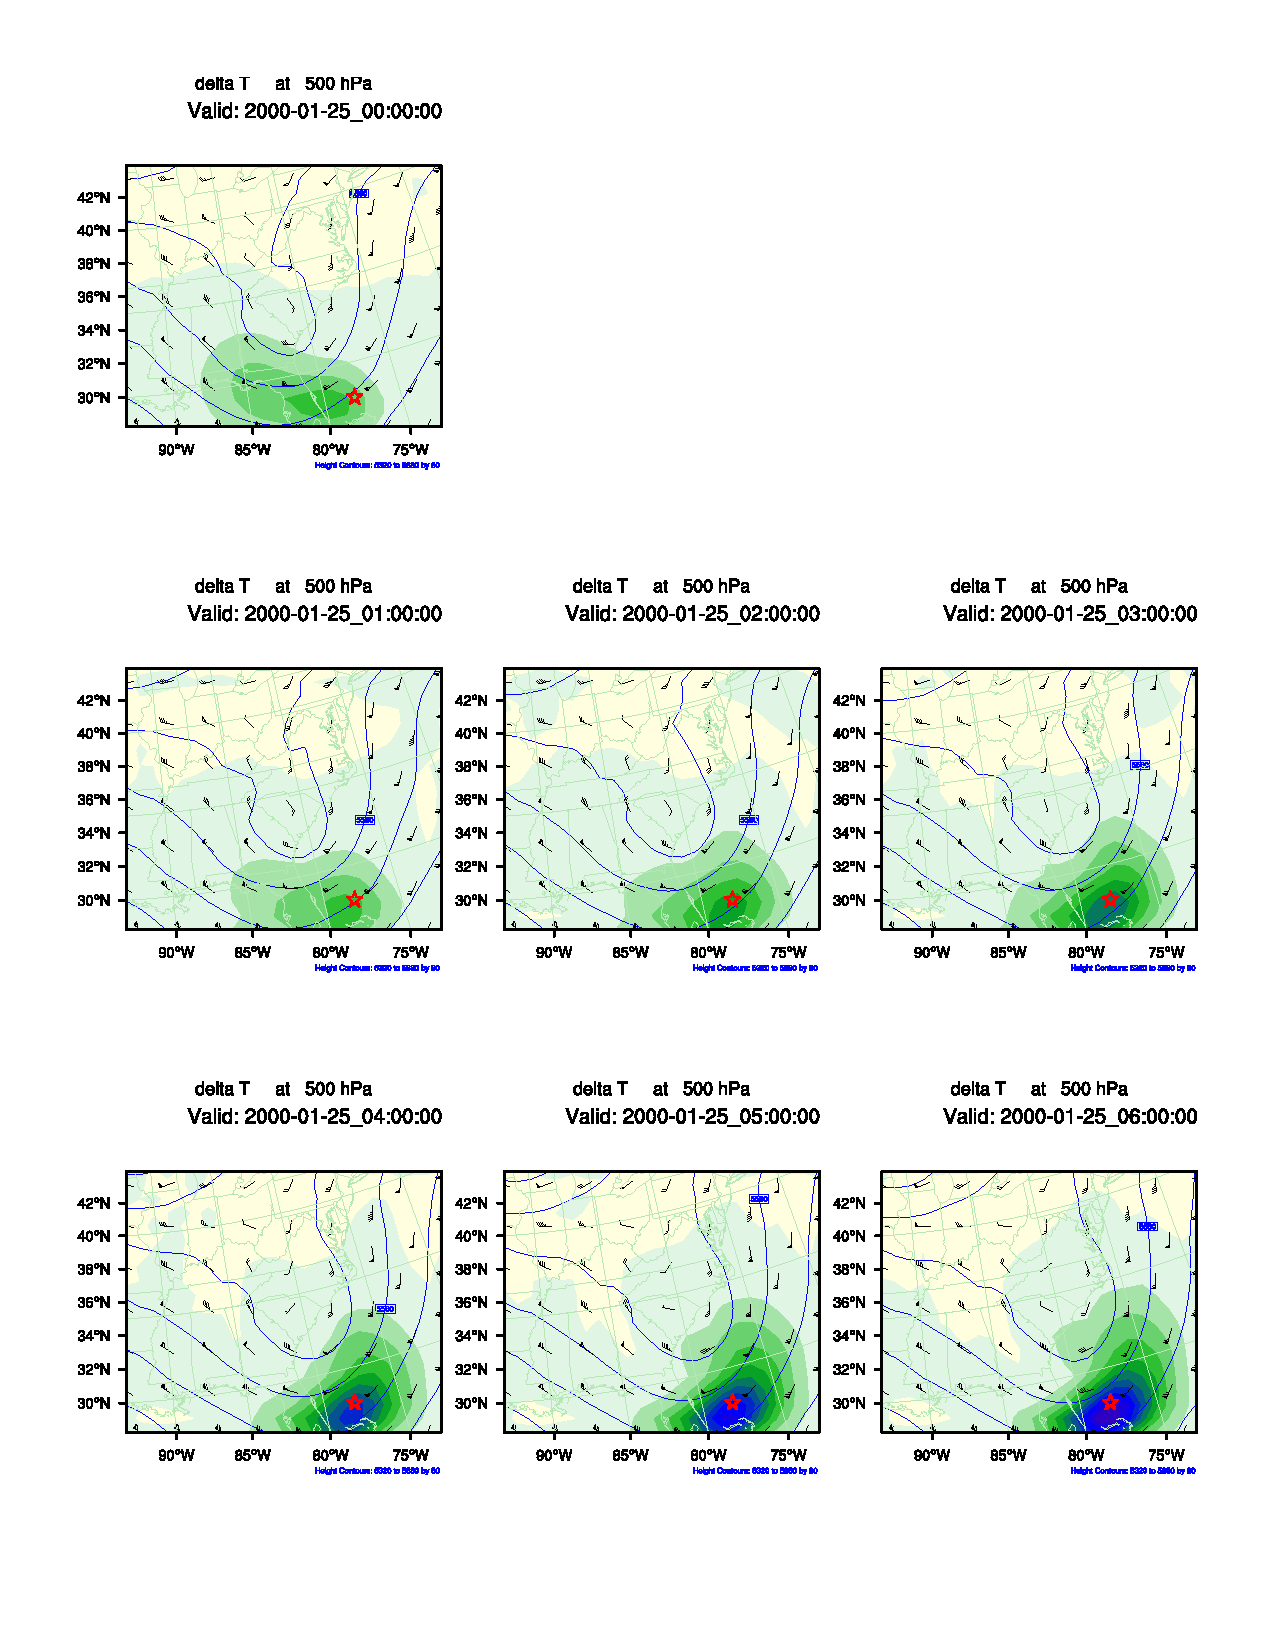
\includegraphics[scale=0.7]{./figures/lbc}
\caption{Evolution of 500hPa potential temperature perturbation with LBC control.}\label{fig:lbc}
\end{figure}

\begin{figure}[t]
\noindent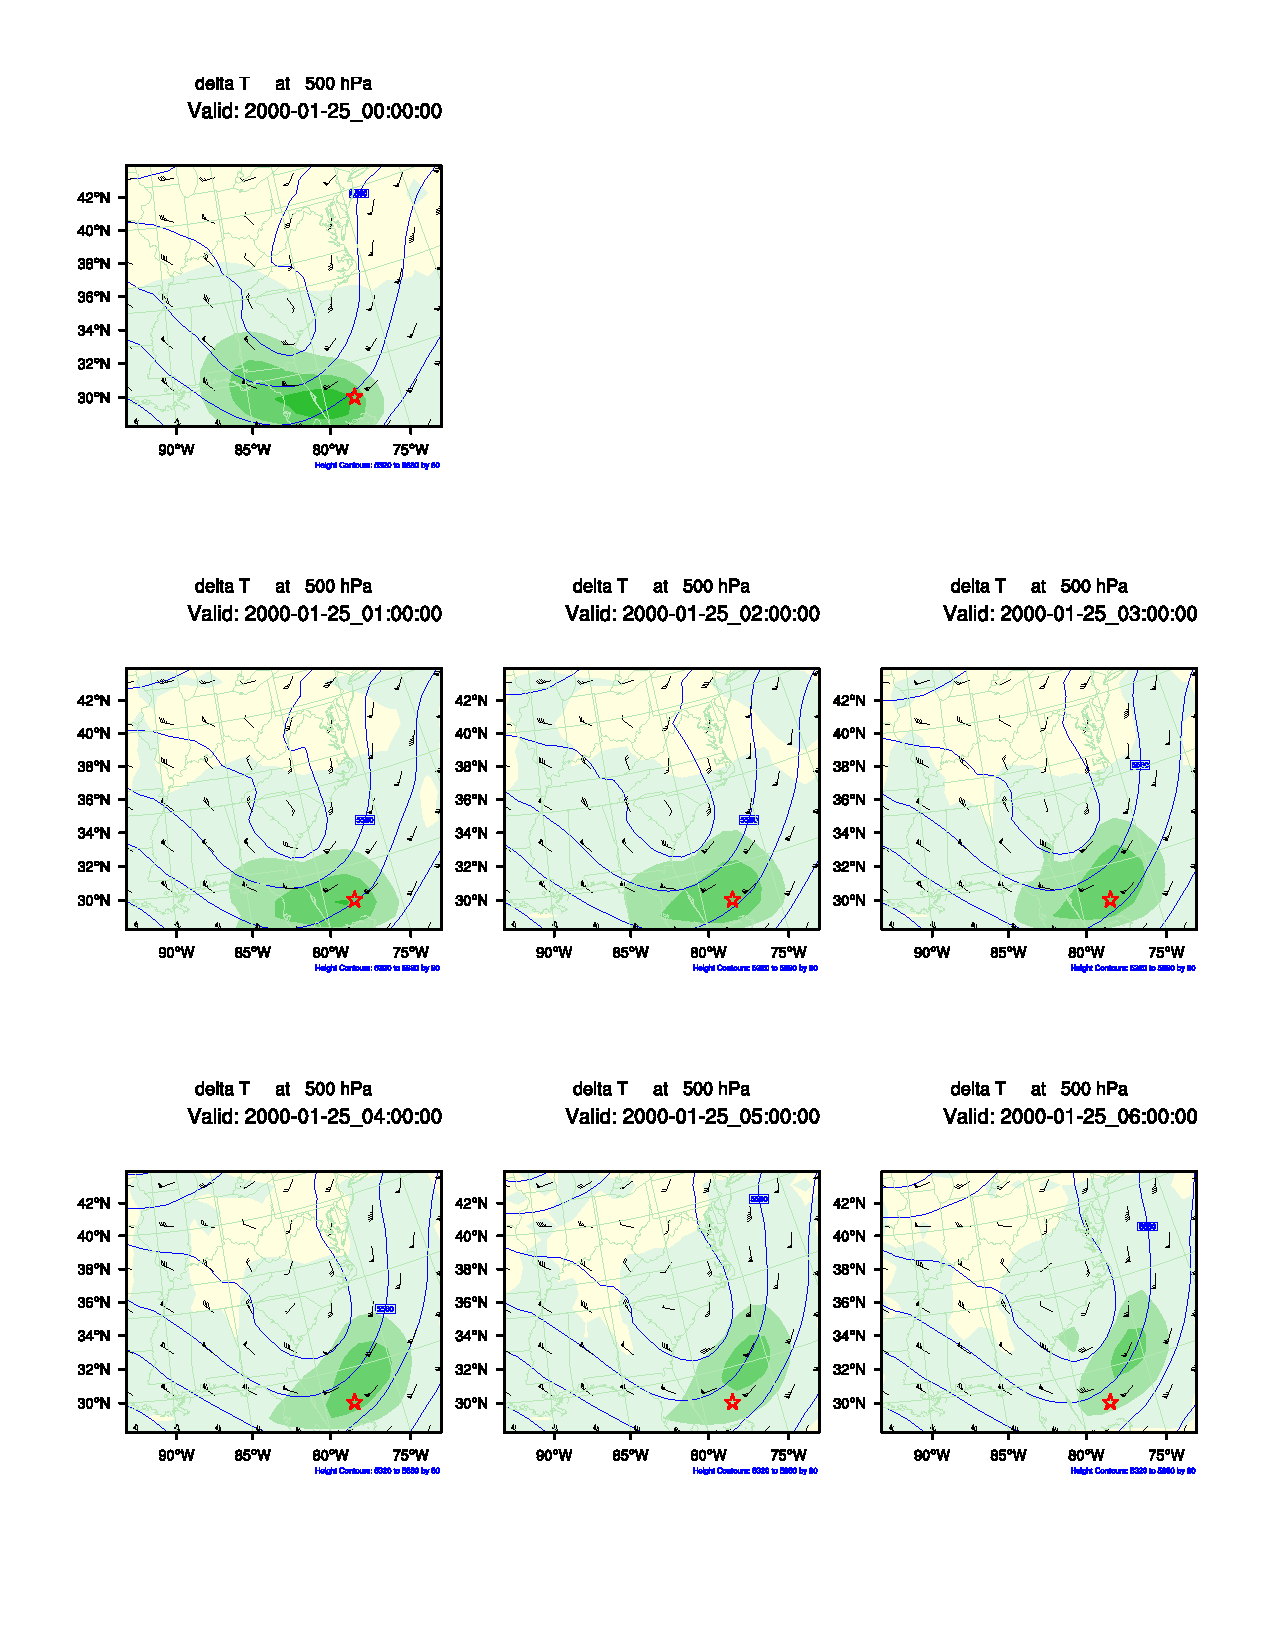
\includegraphics[scale=0.7]{./figures/nolbc}
\caption{Evolution of 500hPa potential temperature perturbation without LBC control.}\label{fig:nolbc}
\end{figure}

\section{Real data experiment}


\section{Conclusion}



%%%%%%%%%%%%%%%%%%%%%%%%%%%%%%%%%%%%%%%%%%%%%%%%%%%%%%%%%%%%%%%%%%%%%
% ACKNOWLEDGMENTS
%%%%%%%%%%%%%%%%%%%%%%%%%%%%%%%%%%%%%%%%%%%%%%%%%%%%%%%%%%%%%%%%%%%%%

\begin{acknowledgment}
The National Center for Atmospheric Research is sponsored by the National
Science Foundation.  This work was supported by the Air Force Weather Agency.
\end{acknowledgment}


%%%%%%%%%%%%%%%%%%%%%%%%%%%%%%%%%%%%%%%%%%%%%%%%%%%%%%%%%%%%%%%%%%%%%
% REFERENCES
%%%%%%%%%%%%%%%%%%%%%%%%%%%%%%%%%%%%%%%%%%%%%%%%%%%%%%%%%%%%%%%%%%%%%
% Create a bibliography directory and place your .bib file there.
\ifthenelse{\boolean{dc}}
{}
{\clearpage}
\bibliographystyle{ametsoc}
\bibliography{../bibliography/references}

\end{document}
%%%%%%%%%%%%%%%%%%%%%%%%%%%%%%%%%%%%%%%%%%%%%%%%%%%%%%%%%%%%%%%%%%%%%
% END OF TEMPLATE
%%%%%%%%%%%%%%%%%%%%%%%%%%%%%%%%%%%%%%%%%%%%%%%%%%%%%%%%%%%%%%%%%%%%%
